\documentclass[usenames,dvipsnames,handout]{beamer}
\usetheme{Frankfurt}
\usecolortheme{default}
\usepackage[utf8x]{inputenc}
\usepackage{lmodern}
\usepackage{amsmath}
\usepackage{amsthm}
\usepackage{amssymb}
\usepackage{enumerate}
\usepackage{mathtools}
\usepackage{xcolor}
\usepackage{tikz}
\usepackage{graphicx}
\usepackage{upgreek}
% \usepackage[sfdefault]{FiraSans}
\usepackage[T1]{fontenc}

\definecolor{main}{RGB}{0, 137, 207}
\definecolor{background}{RGB}{255, 255, 255}
% \setbeamercolor{normal text}{fg=black, bg=background}

\usepackage{color}
\definecolor{keywordcolor}{rgb}{0.7, 0.1, 0.1}   % red
\definecolor{commentcolor}{rgb}{0.4, 0.4, 0.4}   % grey
\definecolor{symbolcolor}{rgb}{0.0, 0.1, 0.6}    % blue
\definecolor{tacticcolor}{rgb}{0.0, 0.1, 0.6}    % blue
\definecolor{sortcolor}{rgb}{0.1, 0.5, 0.1}      % green
\definecolor{stringcolor}{rgb}{0.5, 0.3, 0.2}    % brown
\definecolor{backgroundcolor}{RGB}{230, 230, 230}    % light gray

\usepackage{listings}
\def\lstlanguagefiles{lstlean.tex}
\lstset{language=lean, mathescape=true, backgroundcolor=\color{backgroundcolor}}
\newcommand{\lean}[1]{\lstinline[language=lean]{#1}}
\newcommand{\A}{\mathcal{A}}
\newcommand{\B}{\mathcal{B}}
\newcommand{\C}{\mathcal{C}}

\usetikzlibrary{shapes.misc}
\title{Theorem Proving and Lean}
\author{Bhavik Mehta}
\institute{Bernoulli Center}
\date[\today]{\today}

% \AtBeginSection[]
% {
%   \begin{frame}
%     \frametitle{Outline}
%     \tableofcontents[currentsection]
%   \end{frame}
% }

\begin{document}

\begin{frame}
  \titlepage
\end{frame}

\section{Outline}
\begin{frame}
  \begin{itemize}[<+->]
  \item How we got here
  \item Introduction to Lean
  \item Writing simple proofs in Lean
  \item Writing difficult proofs in Lean
  \end{itemize}
\end{frame}
\begin{frame}
  \begin{itemize}[<+->]
    \item History of automated reasoning
    \item Interactive proving and formal verification
    \item AI for mathematics
    \item Recently formalised combinatorics
  \end{itemize}
\end{frame}
\section{History}
\subsection{}
\begin{frame}{Prehistory}
  \begin{itemize}[<+->]
    \item Principia Mathematica, Whitehead and Russell, 1910s, derive mathematical expressions from a minimal set of axioms
    \item Presburger arithmetic, 1929, natural numbers with addition and equality
    \item G\"{o}del Incompleteness, 1931
    \item Logic Theorist, 1956, could prove around 38 of its first 52 theorems
    \item Automath, 1967, de Bruijn
  \end{itemize}
\end{frame}
\begin{frame}{Restricting the logic}
  \begin{itemize}[<+->]
    \item Propositional logic is decidable
    \item DPLL algorithm, SAT solvers
      \begin{itemize}
        \item Boolean Pythagorean triples
        \item Schur number
      \end{itemize}
    \item First order logic is semi-decidable: you can sometimes make progress (Prover9, Vampire)
    \item Equational logic, eg Robbins conjecture. If $\lor$ is commutative and associative, does $\lnot (\lnot (a \lor b) \lor \lnot (a \lor \lnot b)) = a$ imply we have a Boolean algebra? Yes, EQP 1996.
  \end{itemize}
\end{frame}
\begin{frame}{Special-purpose algorithms}
  \begin{itemize}[<+->]
      \item Four colour theorem (1976) with 1834 configurations to check
      \item Kepler conjecture (2000s), 100,000 linear programs to check
      \item Is the Lorenz attractor strange? Interval arithmetic proof
      \item Rubik's cubes, Sudokus
      \item Computer algebra systems
  \end{itemize}
\end{frame}
\section{Formal verification}
\subsection{}
\begin{frame}{General purpose}
  \begin{itemize}[<+->]
    \item Switch to \emph{interactive} theorem proving in an expressive language
    \item Can formally verify much more, at the cost of less automation
    \item Many but not all systems inspired by Automath
    \item \emph{All} have a `kernel', small but trusted code-base
  \end{itemize}
\end{frame}
\begin{frame}{Some successes}
  \begin{itemize}
    \item Four colour theorem, Coq, 2005
    \item Odd order theorem, Coq, 2012
    \item Kepler conjecture, HOL Light + Isabelle, 2014
    \item Independence of continuum hypothesis, Lean, 2019
  \end{itemize}
\end{frame}
\subsection{Why?}
\begin{frame}{Explaining and learning mathematics}
  \begin{itemize}[<+->]
    \item Allowing the reader to choose their level of detail: a dynamic proof document
    \item Can go all the way to the axioms, if you really want
    \item Can modify an explanation or statement and ensure nothing breaks
    \item Allows the writer to fix assumed background knowledge
    \item Allows the writer to focus on exposition, and let the formal version focus on rigour
    \item Easier to search?
  \end{itemize}
\end{frame}
\begin{frame}{Creating mathematics}
  \begin{itemize}[<+->]
    \item Change your definitions and see how the proof needs to change (optimise the constants more easily!)
    \item Which hypotheses are really needed? How do the lemmas really depend on each other?
    \item Encourages simplifying arguments: asymptotics for cap-set
    \item Encourages powerful abstractions
  \end{itemize}
\end{frame}
\begin{frame}{Collaboration and fun}
  \begin{itemize}[<+->]
    \item Easier to coordinate when you're precise
    \item Contribute with a lower barrier to entry
    \item Liquid Tensor Experiment (Commelin, Scholze)
    \item Polynomial Freiman-Ruzsa (Tao)
    \item Addictive video game
  \end{itemize}
\end{frame}
\begin{frame}{Correctness}
  \begin{itemize}[<+->]
    \item A formally verified proof is correct!
    \item No missing corner cases in your lemma
    \item The definition which is nice enough to prove Lemma 2 is strong enough to be useful in Theorem 6
    \item It's okay that the paper you reference uses different conventions and notation
  \end{itemize}
\end{frame}
\begin{frame}{Many more!}
  \begin{itemize}[<+->]
    \item \emph{Why formalize mathematics?}, Patrick Massot,
    \item \emph{Mathematics and the formal turn}, Jeremy Avigad
  \end{itemize}
\end{frame}
\section{AI for mathematics}
\subsection{}
\begin{frame}
  What about machine learning!
\end{frame}
\begin{frame}{Computers for formulating conjectures}
  \begin{itemize}[<+->]
   \item Tables of primes were used to conjecture the prime number theorem
   \item Tables of elliptic curves were by Birch and Swinnerton-Dyer
   \item OEIS
  \end{itemize}
\end{frame}
\begin{frame}{Generating ideas}
    \begin{figure}
      \centering
      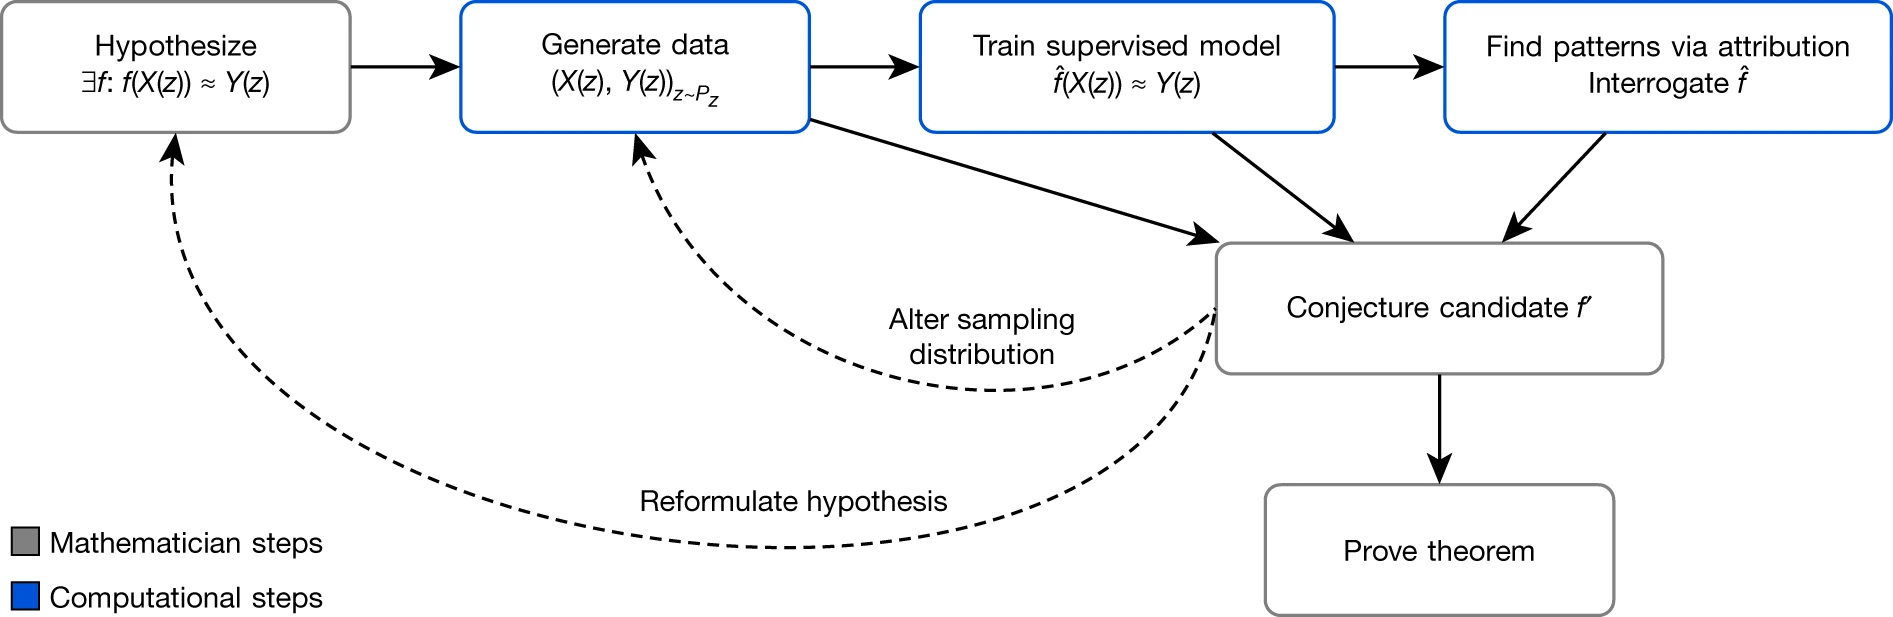
\includegraphics[width=\textwidth]{davies_flowchart.png}
    \end{figure}
    Relate algebraic and geometric invariants in knot theory; new formula for Kazhdan-Lutzig polynomials in representation theory\footnote{Advancing mathematics by guiding human intuition with AI, Alex Davies et al.}
\end{frame}
\begin{frame}{Finding examples}
  \begin{itemize}[<+->]
    \item Adam Wagner, reinforcement learning to find counterexamples to a number of graph theory conjectures\footnote{Constructions in combinatorics via neural networks}
    \item Romera-Paredes, et al, found large 3AP-free sets in $F_{3}^n$ for fixed $n$ (and these tensor)\footnote{Mathematical discoveries from program search with large language models}
    \vspace{3mm}
    \item But these are all discrete, finite objects!
    \item If only we had an expressive computer language for maths which can encode proofs and check them...
  \end{itemize}
\end{frame}
\begin{frame}{AlphaProof}
  \begin{figure}
    \centering
    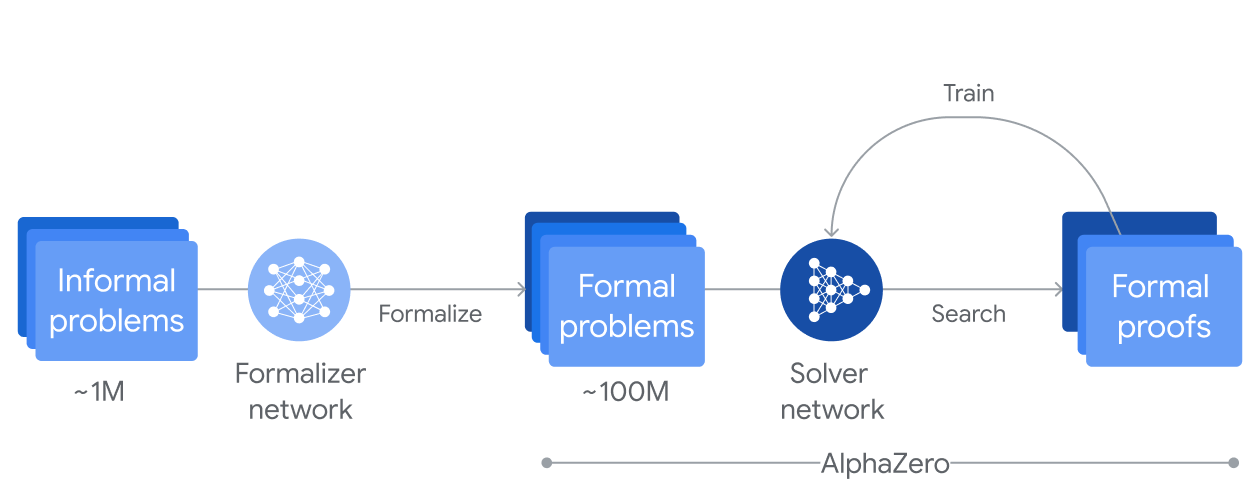
\includegraphics[width=\textwidth]{alphaproof.png}
  \end{figure}
  \url{http://dpmd.ai/imo-silver}
  This system fully solved, in Lean, 3 out of 5 IMO problems
\end{frame}
\section{Combinatorics in Lean}
\subsection{}
\begin{frame}{What is Lean?}
  \begin{itemize}[<+->]
    \item Lean is an open source interactive proof assistant
    \item Written by Leonardo de Moura and his team at Microsoft Research
    \item Lean is a dependently-typed programming language
    \item Very young and very fast growing
    \vspace{3mm}
    \item Emphasis on classical mathematics, and a single library mathlib
    \item A more concrete description coming up!
  \end{itemize}
\end{frame}
\begin{frame}{Additive combinatorics}
  \begin{itemize}[<+->]
    \item Cap-set problem (Dahmen et al)
    \item Solymosi sum-product $\frac{1}{5}|A|^{\frac{5}{4}} \leq \max |A+A|, |AA|$ (M.)
    \item Szemer\'{e}di's regularity lemma and $r_{3}(N) = o(N)$ (Dillies, M.)
    \item $N / \exp(4 \sqrt{\log N}) \leq r_{3}(N) \leq N / \log \log N$ (M.)
    \item Pl\"{u}nnecke-Ruzsa inequality (Dillies)
    \item Erd\H{o}s-Graham problem (Bloom, M.)
  \end{itemize}
\end{frame}
\begin{frame}{Highlights}
  \begin{itemize}[<+->]
    \item $R(k) \leq (4 - \varepsilon) ^ k$ (M.)
    \item Proved in March 2023, 57 page long paper, one person, formalised in 5 months
      \vspace{3mm}
    \item Polynomial Freiman-Ruzsa (Tao)
    \item Proved in December 2023, 20 page long proof, around 30 people contributed, formalised in \emph{three weeks}
  \end{itemize}
\end{frame}

\begin{frame}{But what really is Lean?}
  Aims:
  \begin{itemize}
    \item Understanding the language and basics of Lean
    \item How to actually use Lean to prove simple things
    \item How to use Lean for more practical things
  \end{itemize}
\end{frame}

\end{document}

